\documentclass{article}
\usepackage{amsfonts,amsmath,amssymb,listings,graphicx}

\setlength{\oddsidemargin}{.25in}
\setlength{\evensidemargin}{.25in}
\setlength{\textwidth}{6.25in}
\setlength{\topmargin}{-0.4in}
\setlength{\textheight}{8.5in}

\author{2012 ACM Class 5120309027 Huang Zen}
\title{Problem Set 2}
\date{}

\begin{document}
\maketitle
\paragraph{1.}
Let's suppose the probability that one tests positive is $p$,
independently. Let $X_i$ be the indicator variable when $X_i=1$ means
person $i$ tests positive and $X_i=0$ means not. Let $Y_i,1\leq i\leq 4$
be the indicator variable when $Y_i=1$ means group $i$ tests positive.
So that $X = \displaystyle \sum_{i=1}^{n} X_i + \sum_{i=1}^{4} Y_i + 2$ is
the variable of all the tests performed. $X_i=1$ occurs only when
there is at least one person testing positive in person $i$'s nearby
$n/4$ group. So 
$$ E(X_i) = P(X_i=1) = 1 - (1-p)^\frac{n}{4} $$
$$ E(Y_i) = P(Y_i=1) = 1 - (1-p)^\frac{n}{2} $$
when
\begin{align*}
E(X) &= \sum_{i=0}^{n} E(X_i) \\
     &= n + 6 - n (1-p)^\frac{n}{4} - 4 (1-p)^\frac{n}{2}
\end{align*}
Compare $E(X)$ to $n$, we found when $p <
\sqrt[\frac{n}{4}]{\frac{-n+\sqrt{n^2+96}}{8}}$, $E(X) < n$.
\\
for $m$ groups scheme, we have
$$
E_{m,k}(X) = m + n - n (1-p)^k
$$


\paragraph{2.}
Let $A$ be the event that the hand has an ace, $RA$ be the event that
the hand has an ace of hearts. we have
\begin{align*}
P(A) = 1 - \frac{C^{13}_{48}}{C^{13}_{52}} &= 0.6962 \\
P(RA) = \frac{C^{12}_{51}}{C^{13}_{52}} &= 0.2500
\end{align*}
Let $AA$ be the event that the hand has two or more aces, $RAA$ be the event
that the hand has two or more aces and one is hearts. we have
\begin{align*}
P(AA) &= 1 - \frac{C^{13}_{48}}{C^{13}_{52}} -
\frac{4C^{12}_{48}}{C^{13}_{52}} = 0.2573 \\
P(RAA) &= \frac{C^{12}_{51}-C^{12}_{48}}{C^{13}_{52}} = 0.1403
\end{align*}
Now that
\begin{align*}
P(AA | A) &= \frac{P(AA)}{P(A)} = 0.3696\\
P(RAA | RA) &= \frac{P(RAA)}{P(RA)} = 0.5612
\end{align*}
So the two probabilities are not equal.

\paragraph{3.}
Let's calculate the convarince of $X+Y$ and $X-Y$ to see whether they
are independent. Let $u = X+Y$ and $v = X-Y$, we have
\begin{align*}
con(u,v) &= E(uv) - E(u)E(v) \\
         &= E(X^2 - Y^2) - E(X+Y)E(X-Y) \\
         &= E(X^2) - E(Y^2) - E^2(X) + E^2(Y) \\
         &= Var(X) - Var(Y)
\end{align*}
since normal random variables $X$ and $Y$ have the same parameter
$\sigma ^2$, $Var(X) = Var(Y)$, so 
$$
con(u,v) = 0
$$
which shows that $X$ and $Y$ are independent.

\paragraph{4.}
If the generating throws a result of $X = k$, it must be
$\displaystyle \sum_{0}^{k-1}p_i \leq U < \sum_{0}^{k}p_i $, which means $U$ falls
in an interval of length $p_k$. Since $U$ is a uniform random
variable, this has a probabilty of $p_k$, so the generating works.
\\
The matlab code for random generating and plot is here:
\
\begin{lstlisting}[language=matlab,numbers=left]
function [] = genepossion
    lamda=5;
    times=1000;
    function [ out ] = gene( u, lamda )
        out=0;
        p=exp(-lamda);
        while(u>p)
           out=out+1; 
           u=u-p;
           p=p*lamda/out;
        end
    end
    list=rand(1,times);
    for t=1:times
        genelist(1,t)=gene(list(1,t),5);
    end
    gmin=min(genelist);
    gmax=max(genelist);
    gp=linspace(gmin,gmax,20);
    f=ksdensity(genelist,gp);
    plot(gp,f);
end
\end{lstlisting}
The distribution graphy is here:
\\
\scalebox{0.50}{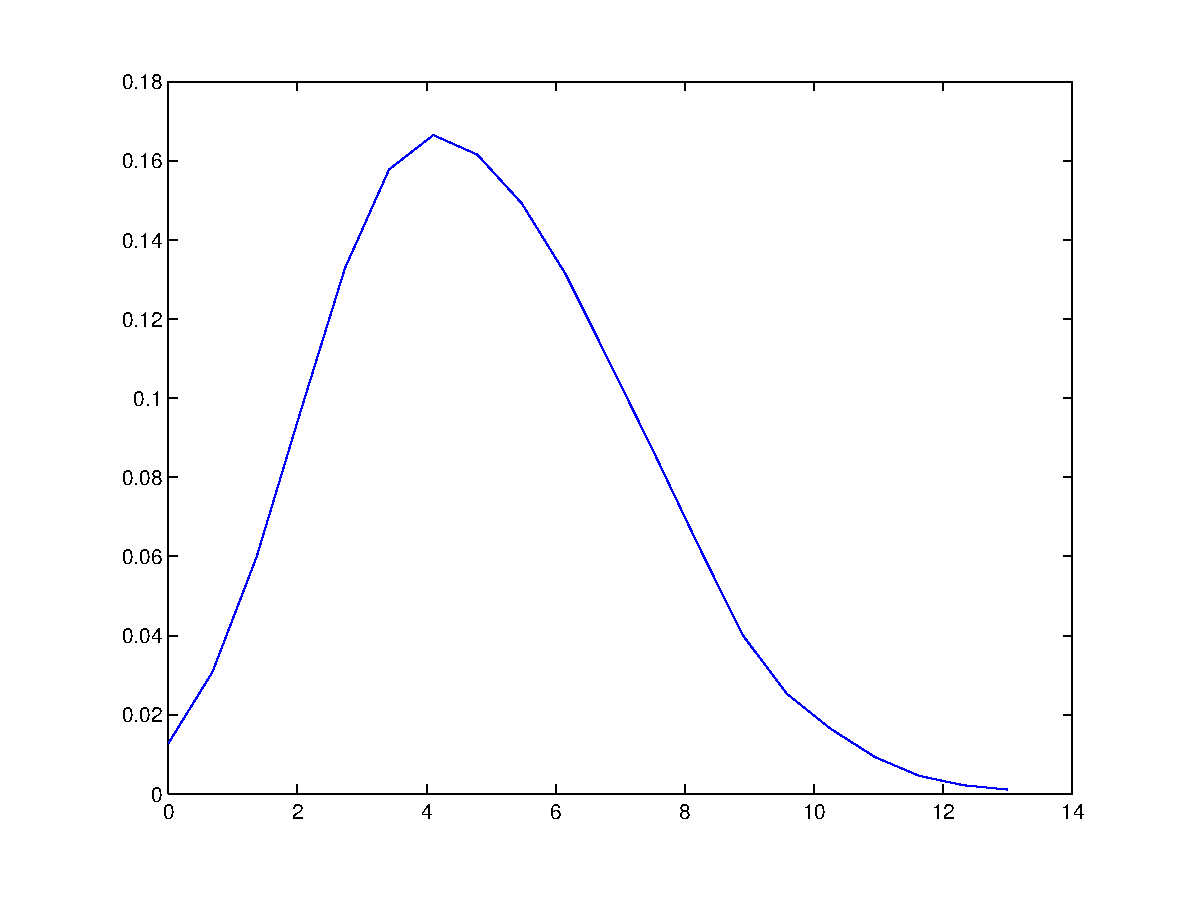
\includegraphics{PS2.eps}}
\end{document}
